%!TEX root = ../Thesis.tex

\section{Trilateration}
Unlike triangulation, which uses the angles from known points, trilateration uses the distances from known points. This is the base concept behind GNSS. Satellite W sends out a radio signal at time X and it's position Y which the user received at time Z. The time difference is used to calculate the distance from the satellite's position. With this information from multiple satellites, the users position is calculated.



- timing comparison between satellite and receiver to find psudeorange
- ECEF frame of reference

\begin{figure}
\centering
\caption{}
\label{fig:trilateration}
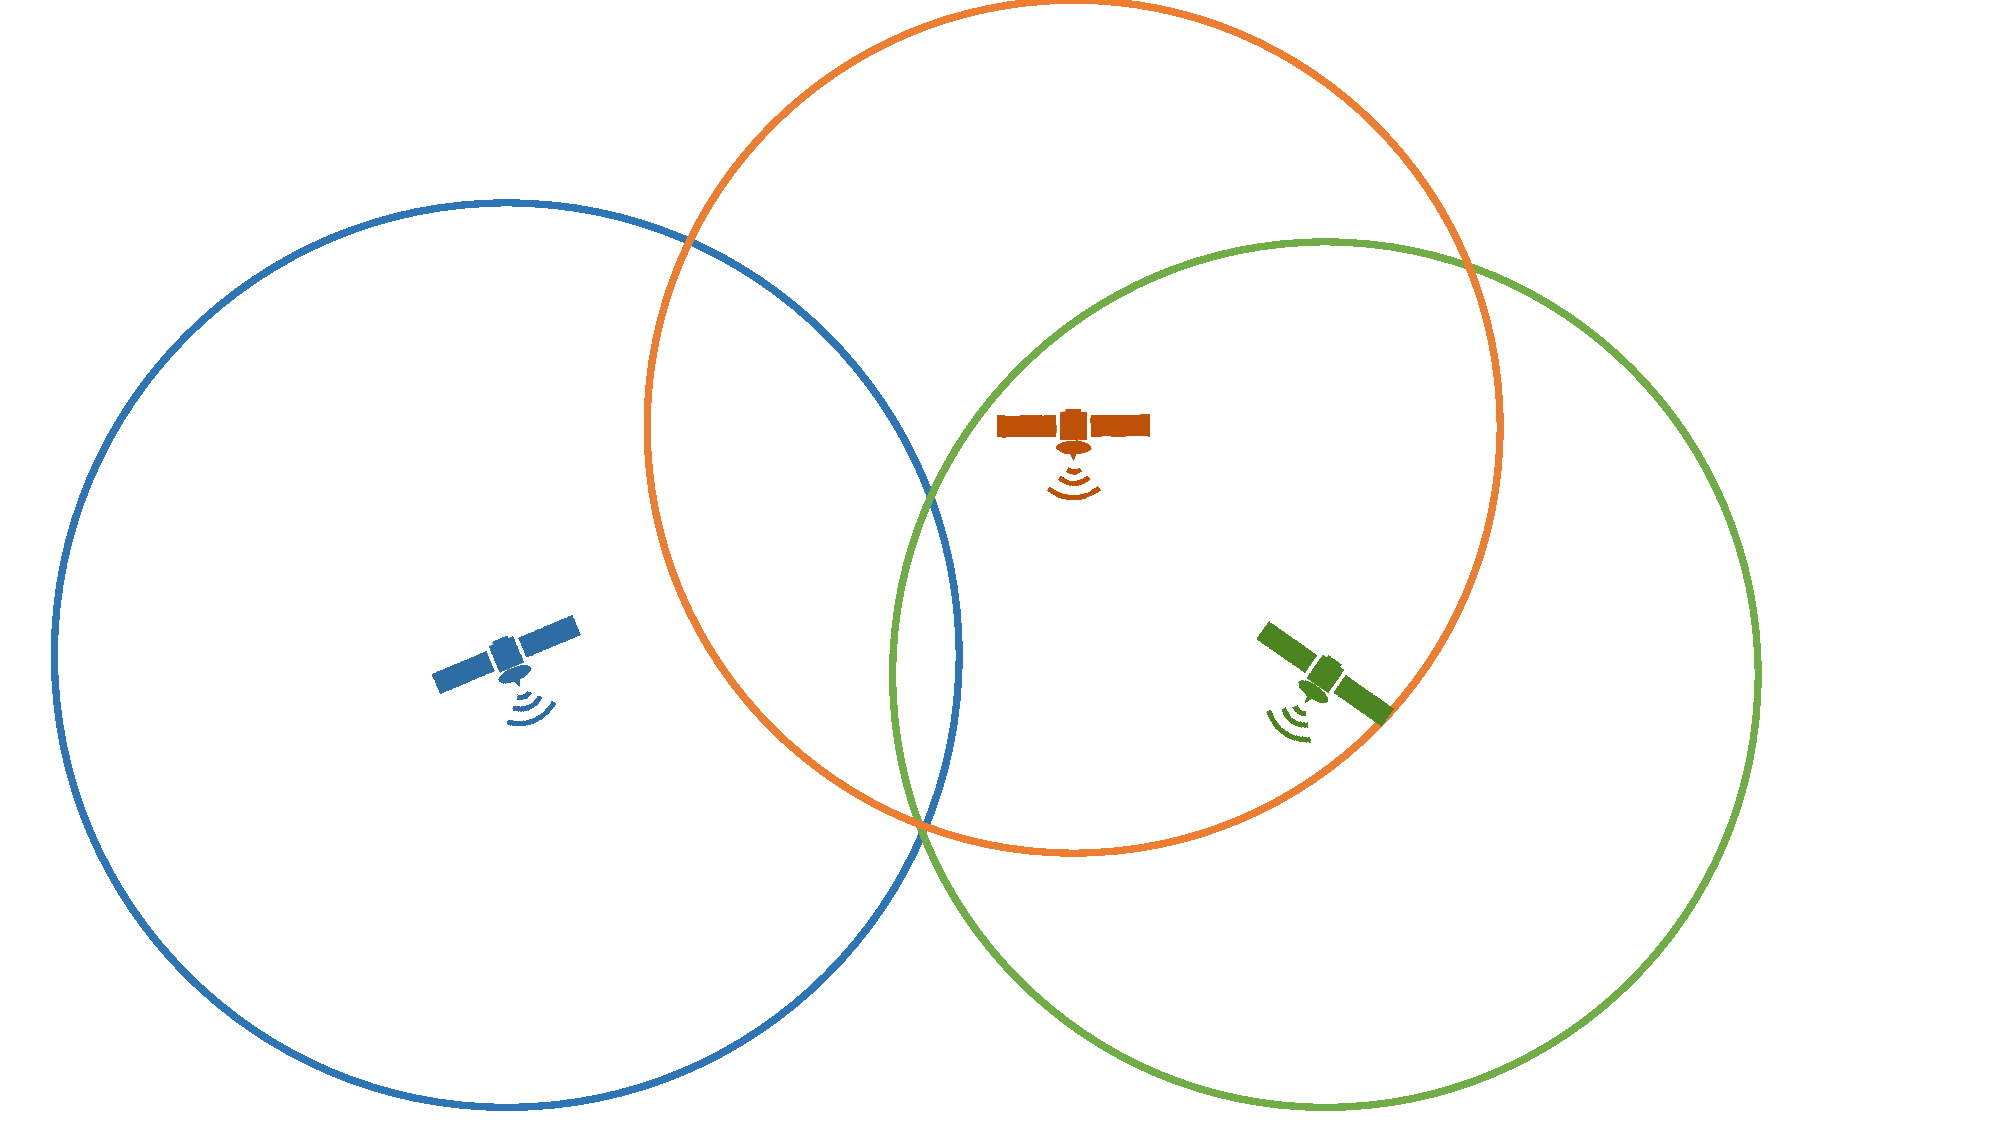
\includegraphics[width=0.7\linewidth]{ChapterLiteratureReview/trilateration}
\end{figure}

\begin{figure}
\centering
\caption{}
\label{fig:trilaterationtime}
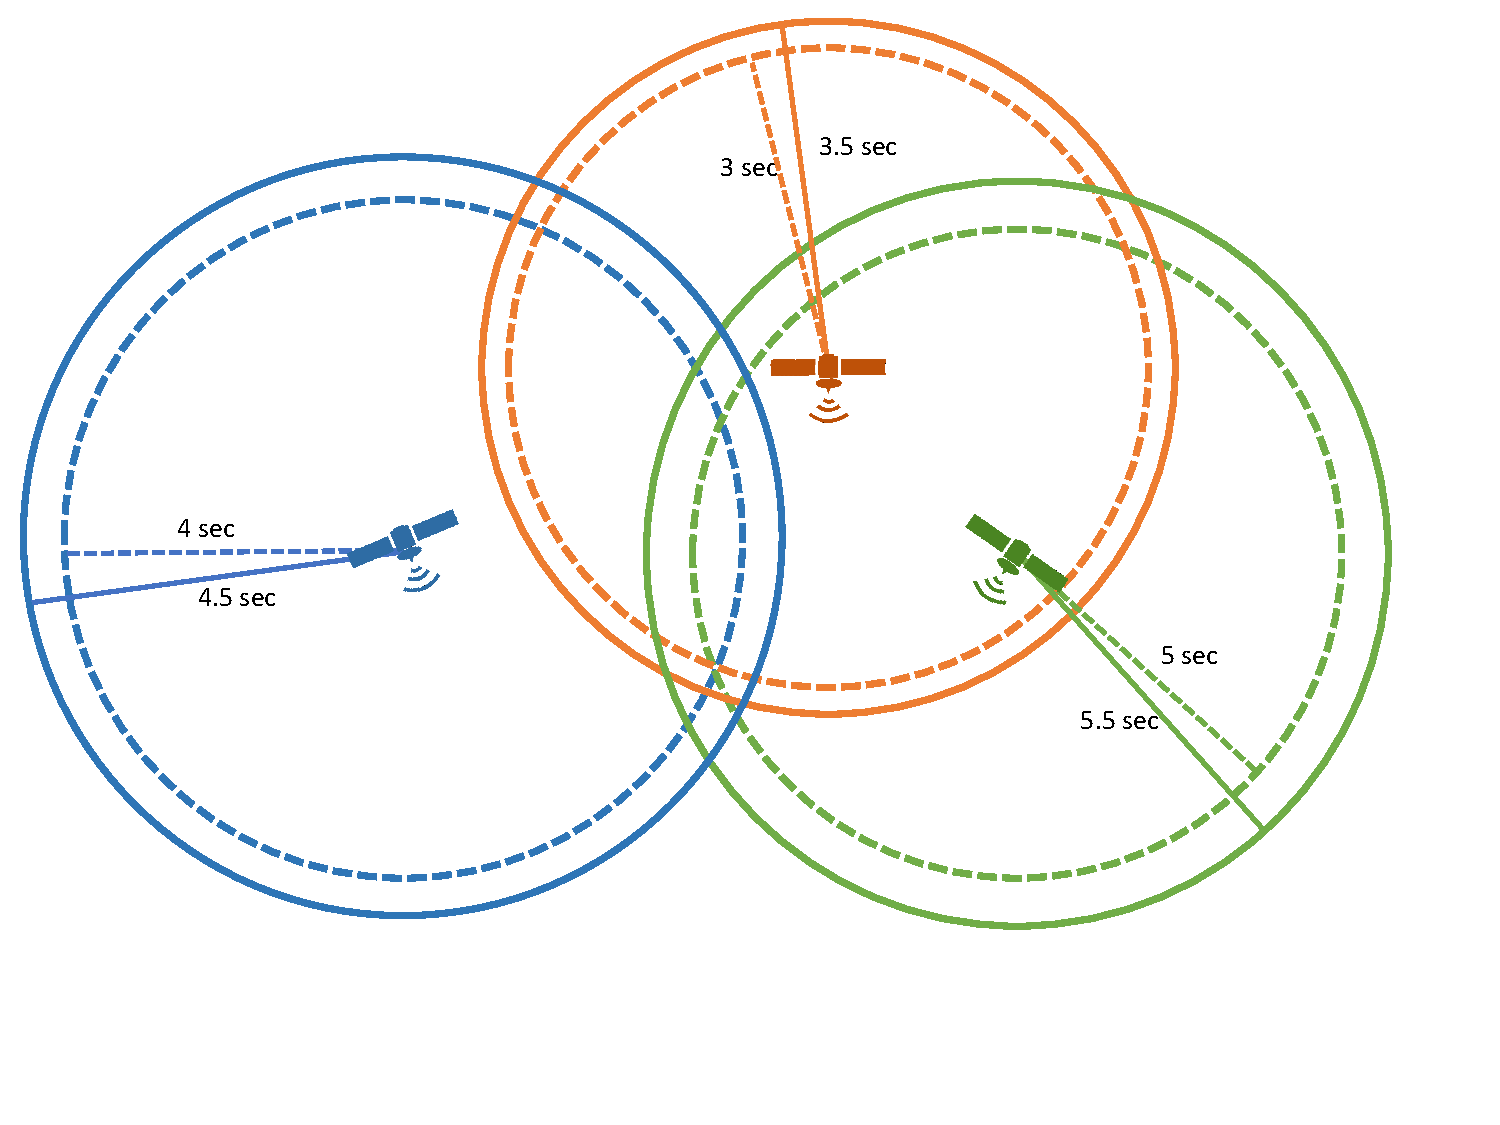
\includegraphics[width=0.7\linewidth]{ChapterLiteratureReview/trilaterationtime}
\end{figure}







- NLLS solve spheres
- need 4 satellites minimum
- 
